% S2: Audit Validity for Fairness Metrics.
%
% Five things are bound here because none of them is a claim about this
% thesis's clinical contradiction detector and none is read sequentially
% against the chapters that summarise them: the literature's own warning
% that a disaggregated evaluation needs assumptions about the selection
% mechanism it is applied under; the degeneracy precondition that a
% parity-style audit must clear before it produces a substantive number;
% the sign-provenance defect in how a disparity gap was stored and the
% retrofit that recovered direction without changing any previously
% reported magnitude; the unexplained selection-channel anomaly, reported
% as an anomaly rather than as a finding; and the full quantitative record
% behind that anomaly, bound in full immediately afterwards rather than left
% to a reader's trust. Numbers and claims are unchanged from the thesis
% chapters and the appendix file they were moved from; only cross-references
% have been adjusted for the move, as noted at each site.

\section{Audit Validity for Fairness Metrics}
\label{sup:s2}

\subsection{Disaggregated evaluation and what it assumes}

\citet{barocas2021disaggregated} lay out the design choices in evaluating an AI system across
demographic groups and argue they are consequential enough to require documentation, since
they shape both what is measured and its effect on the populations measured.
\citet{pfohl2025disaggregated} sharpen the warning: when a dataset faithfully reflects a
population that already contains disparities, equal performance across groups does not
indicate the absence of a problem, and when data are unrepresentative through selection bias,
both disaggregated evaluation and conditional-independence alternatives may be invalid without
explicit assumptions about the selection mechanism. \citet{fogliato2020fairness} make the
parallel point about the label rather than the sample: when the observed outcome is a biased
proxy for the outcome of interest, group-wise differences measured against the proxy need not
track those against the target, and they offer a sensitivity analysis rather than a
correction. Both results constrain what a measured disparity may be read as.

Those results are why a selection-channel finding cannot be reported as a fairness result
without an accompanying mechanism. Section~\ref{sup:sec:disc-anomaly} reports an unexplained anomaly in
how a pool audit responds to the channel through which items are selected, reported as
unexplained because \citet{pfohl2025disaggregated} establish that interpreting such a pattern
depends on assumptions about the selection mechanism not available here. No subgroup harm is
demonstrated anywhere in this work, and none is claimed.


\subsection{The degeneracy precondition}

\textbf{Condition.} Demographic parity compares the predicted-positive rate across groups, so a
classifier that predicts one class for nearly every input has the same predicted-positive rate in
every group by construction and cannot exhibit a parity disparity, whatever the underlying data. An
audit that reports no disparity on such a classifier is therefore reporting its own operating point,
not a property of the model or of the data it was run against. This is the degeneracy precondition:
a check on the validity of a parity-style audit over a binary classifier, checkable before the audit
runs. It is a precondition, not a general result about fairness metrics, and beyond what the rest of
this chapter already reports it establishes nothing about this thesis's contradiction detector.

The precondition is enforced by two mechanisms, run in order and both before the audit produces any
substantive measurement. First, a pre-registered non-degeneracy bar: the reference classifier must
clear a minimum AUROC of $0.65$, a predicted-positive rate strictly inside the interval $0.05$ to
$0.50$, and a precision lift over the base rate of at least $1.5$, all on the validation split and
all asserted in code before the sweep begins; if any of them fails, the driver exits and the sweep
does not run. Second, a planted-gap positive control, which runs immediately afterwards and checks
that the audit can detect a disparity known to be present: a known logit shift is injected into one
group's scores on the full population with no selection filtering, and the audit code must recover
it, the bootstrap interval on the demographic parity gap must exclude zero and the four-fifths ratio
must fall below its threshold with an interval upper bound below one. If the audit cannot recover a
gap placed there deliberately, every downstream number is void, and the experiment driver aborts
rather than reporting them. The precondition also applies retrospectively to an earlier audit in
this project and fails there, which is why no subgroup harm is demonstrated or claimed anywhere in
this thesis.


\subsection{Sign provenance}
\label{sup:sec:signprov}

Table~\ref{sup:tab:signed} records the recomputation.

The three experiments in this subsection, the selection experiment and the two
PUMS regimes, run on simulated populations rather than the clinical pipeline,
and are retained because the sign-provenance rule they establish was
applied to the clinical numbers reported elsewhere in this thesis.

A second defect concerns direction rather than magnitude. Where a gap statistic
is stored as an absolute value, no directional claim can be recovered afterwards,
and a reader cannot tell which group a reported disparity favours. The signed
re-analysis reproduced the stored values exactly, at a maximum discrepancy of
$0.0$, which establishes that it is a faithful reproduction rather than a
different computation.

\begin{table}[H]
\caption[Signed parity endpoints, three experiments]{Signed demographic parity endpoints in three experiments.}
\centering
\small
\begin{tabular}{lrrl}
\toprule
\textbf{Experiment} & \textbf{Endpoint 1} & \textbf{Endpoint 2} &
\textbf{Sign changes} \\
\midrule
Selection experiment & $0.00841$  & $0.18939$  & none \\
PUMS, regime A       & $-0.13556$ & $-0.19435$ & none \\
PUMS, regime B       & $-0.11807$ & $-0.04101$ & none \\
\bottomrule
\end{tabular}
\apanote{Endpoint 1 is the signed gap at the weakest selection strength swept, Endpoint 2 at the strongest, not the sweep's extrema. On regime A the true minimum and maximum, $-0.20733$ and $-0.12761$, both lie outside the printed endpoints; on regime B the true minimum, $-0.12034$, is more extreme than the printed $-0.11807$, while the true maximum coincides with it. On the selection experiment both printed endpoints are the sweep's own extrema. All endpoints are reported as recorded.}
\label{sup:tab:signed}
\end{table}

The sign analysis establishes that absolute-value storage destroys the
information a directional claim needs and that the three experiments
re-examined do not change sign inside their own sweeps; it demonstrates no
harm to any subgroup, and with 12 positives no subgroup performance claim is
supportable.


\subsection{An Anomaly, Reported as an Anomaly}
\label{sup:sec:disc-anomaly}

One result here is not explained, and this section reports it without
explaining it. It is not counted among the contributions Chapter 1 of the thesis lists, since a contribution earns its place by explaining something
and this pattern explains nothing about itself. The population audited is
simulated, not the clinical pipeline, and is retained because the same
experiments anchor the sign-provenance rule of Section~\ref{sup:sec:signprov},
applied afterward to the clinical numbers, and because a pattern that does
not fit is better reported than dropped.

On two simulated populations, with baseline disparity held fixed, upstream
selection channels were swept and the pool-level demographic parity gap
audited at each step. The gap never changes sign within a sweep, but the
direction it drifts in does: two channels on the same population give fitted
drift slopes of opposite sign, and extending one sweep across operating
points as well as channel strength shows the audited gap moving with both,
so a single audited number describes one cell of a surface rather than the
system that produced it. A further, controlled sweep across baselines,
channel strengths and replicates does not even reproduce that channel
dependence, inverting the mapping between channel and drift direction: the
direction a pool audit drifts in is not a stable function of the channel
that produced it.

Five mechanism claims were proposed during this project to account for this
pattern; each was tested against a parameter sweep and each failed, and a
sixth is not offered. No subgroup harm is demonstrated anywhere in this work,
and no general claim is made that disaggregated fairness evaluation is
uninterpretable under selection; that argument, and the observation that the
design choices inside a disaggregated evaluation are consequential enough to
need documenting, belong to others and predate this work
\citep{pfohl2025disaggregated,fogliato2020fairness,barocas2021disaggregated}.
The full sweep, the operating-point surface, and the failed mechanism
accounts are released with the analysis code rather than bound here.



\subsection{Full Quantitative Treatment of the Selection-Channel Anomaly}

The summary above is the anomaly as this supplement reports it. What follows, reproduced from the appendix that has carried it since it
was first bound, is the full quantitative record behind that summary: the
per-regime signed endpoints, the operating-point surface, and the figure the
summary above refers to only in words.

\begingroup
% msu_appE_anomaly.tex opens with \chapter{...}\label{app:anomaly}. This
% document has no chapter-lettered appendices to house it in, so \chapter is
% suppressed for the extent of this input; the subsection heading above
% already gives the reader the heading \chapter would otherwise have
% printed. \label{app:anomaly} still fires, against whatever section-level
% \@currentlabel is active at that point, and is not relied on by any \ref
% in this document.
\renewcommand{\chapter}[1]{}
% This appendix is bound in the supplement, not the thesis: it is the full
% treatment of the selection-channel anomaly that the thesis's discussion
% chapter reports only in summary, together with a pointer here in words
% (the thesis and this file are separate documents, so a \ref to a label
% defined in one cannot resolve in the other). No citation appears below;
% the citation-bearing sentences about this anomaly stay in the thesis
% chapter, which carries the bibliography this file does not.
\chapter{The Selection-Channel Anomaly: Full Treatment}
\label{app:anomaly}

This appendix gives the full quantitative record behind the anomaly the
thesis's discussion chapter reports in summary: an unexplained pattern in
how a pool-level demographic-parity audit drifts across a swept upstream
selection channel, observed on simulated populations kept separate from the
clinical pipeline, and reported here rather than suppressed because it does
not fit any account offered for it. Nothing in this appendix is claimed as a
contribution; it is the record a reader checking the chapter's summary of
the pattern would need.

On one simulated population, with baseline disparity held fixed, two
upstream selection channels were swept and the pool-level demographic parity
gap audited at each step. Under the first the signed gap runs from
$-0.13556$ to $-0.19435$; under the second, from $-0.11807$ to $-0.04101$.
Neither series changes sign, but the fitted drift slopes have opposite sign,
and neither series is monotone in channel strength, so the endpoints do not
describe the trajectory. Fitted as drift slopes, the two channels produce
signed drifts of opposite sign, $-0.00780$ under the first regime and
$+0.01177$ under the second. A third selection experiment on a different
pool gives a gap running from $+0.00841$ to $+0.18939$, again without a sign
change.

That third experiment was also swept across operating points, and
Figure~\ref{fig:appE-threshold-surface} shows what the sweep returned. The
audited gap is not a property of the system on its own. It moves with the
operating point and with the strength of the upstream selection, so any
single audited number describes one cell of that surface rather than the
system that produced it, and the operating point actually used crosses the
tolerance contour partway along the sweep. Over a large part of the surface
the audit also stops being able to answer at all: where the minimum
detectable gap exceeds the tolerance the audit was written against, a cell
that reads as passing is reporting a sample size rather than a system, and
the two cases are not distinguishable from the recorded pass alone.

\begin{figure}[!ht]

% Caption stays after the graphic in source order: main_supplement.tex's
% \captionsetup[figure]{position=bottom} only sets caption skip amounts, it
% does not reorder the box, so this is what actually puts the caption below
% the figure, matching main_msu.tex's figure convention (author's decision
% of 2026-08-13, recorded there) that the rest of this document follows.
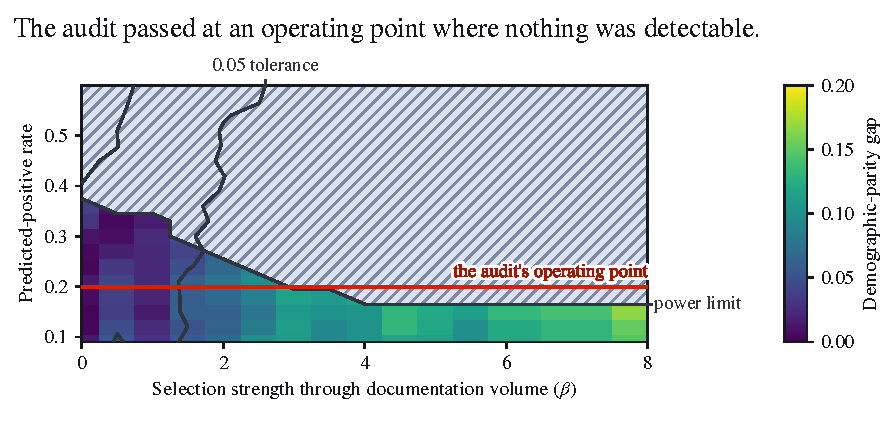
\includegraphics[width=0.98\linewidth]{figures/fig-threshold-surface.pdf}
\caption[Audited parity gap across operating points]{The audited
demographic-parity gap across operating points and selection strengths for
one selection experiment. The solid contour is the tolerance the audit was
written against. The hatched region is where the minimum detectable gap
exceeds that tolerance.}
\label{fig:appE-threshold-surface}
\end{figure}

The behaviour does not survive a controlled sweep of the same construct. A
simulator sweep over baselines, channel strengths and replicates inverts the
mapping between channel and drift direction; the grid's dimensions are not
registered, so none is quoted here. The direction in which a pool audit
drifts is therefore not a stable function of the selection channel that
produced the pool, at least across the region examined.

Five mechanism claims were proposed during this project to account for this.
Each was written down, each was tested against a parameter sweep, and each
failed; the record of those attempts is kept with the thesis's own
correction record, bound as an appendix to the thesis itself rather than
here. A sixth is not offered, and that restraint is a position rather than
an omission. The cheapest move available here is to build a story fitting
the two regimes actually observed. It would be unfalsified, because it would
be assembled after the fact from the data it purports to explain, and in the
write-up it would be indistinguishable from the five that already failed.

The supported claim is narrow and complete: on one population, with
baseline disparity fixed, the sign of the drift in a pool-level parity audit
is channel-dependent in a way a controlled sweep does not reproduce. Anyone
reading a single audited drift as evidence about an upstream selection
process is reading something whose direction was not stable where it was
checked. No subgroup harm is demonstrated, none is demonstrated anywhere in
this work, and these populations are simulated. No boundary for the effect
is claimed either, because the sweep that inverts the mapping is one
simulator with one functional form.

\endgroup
